\section{Receiver Blokken}

\subsection{Lampe (David)}

\begin{figure}[h]
\centering
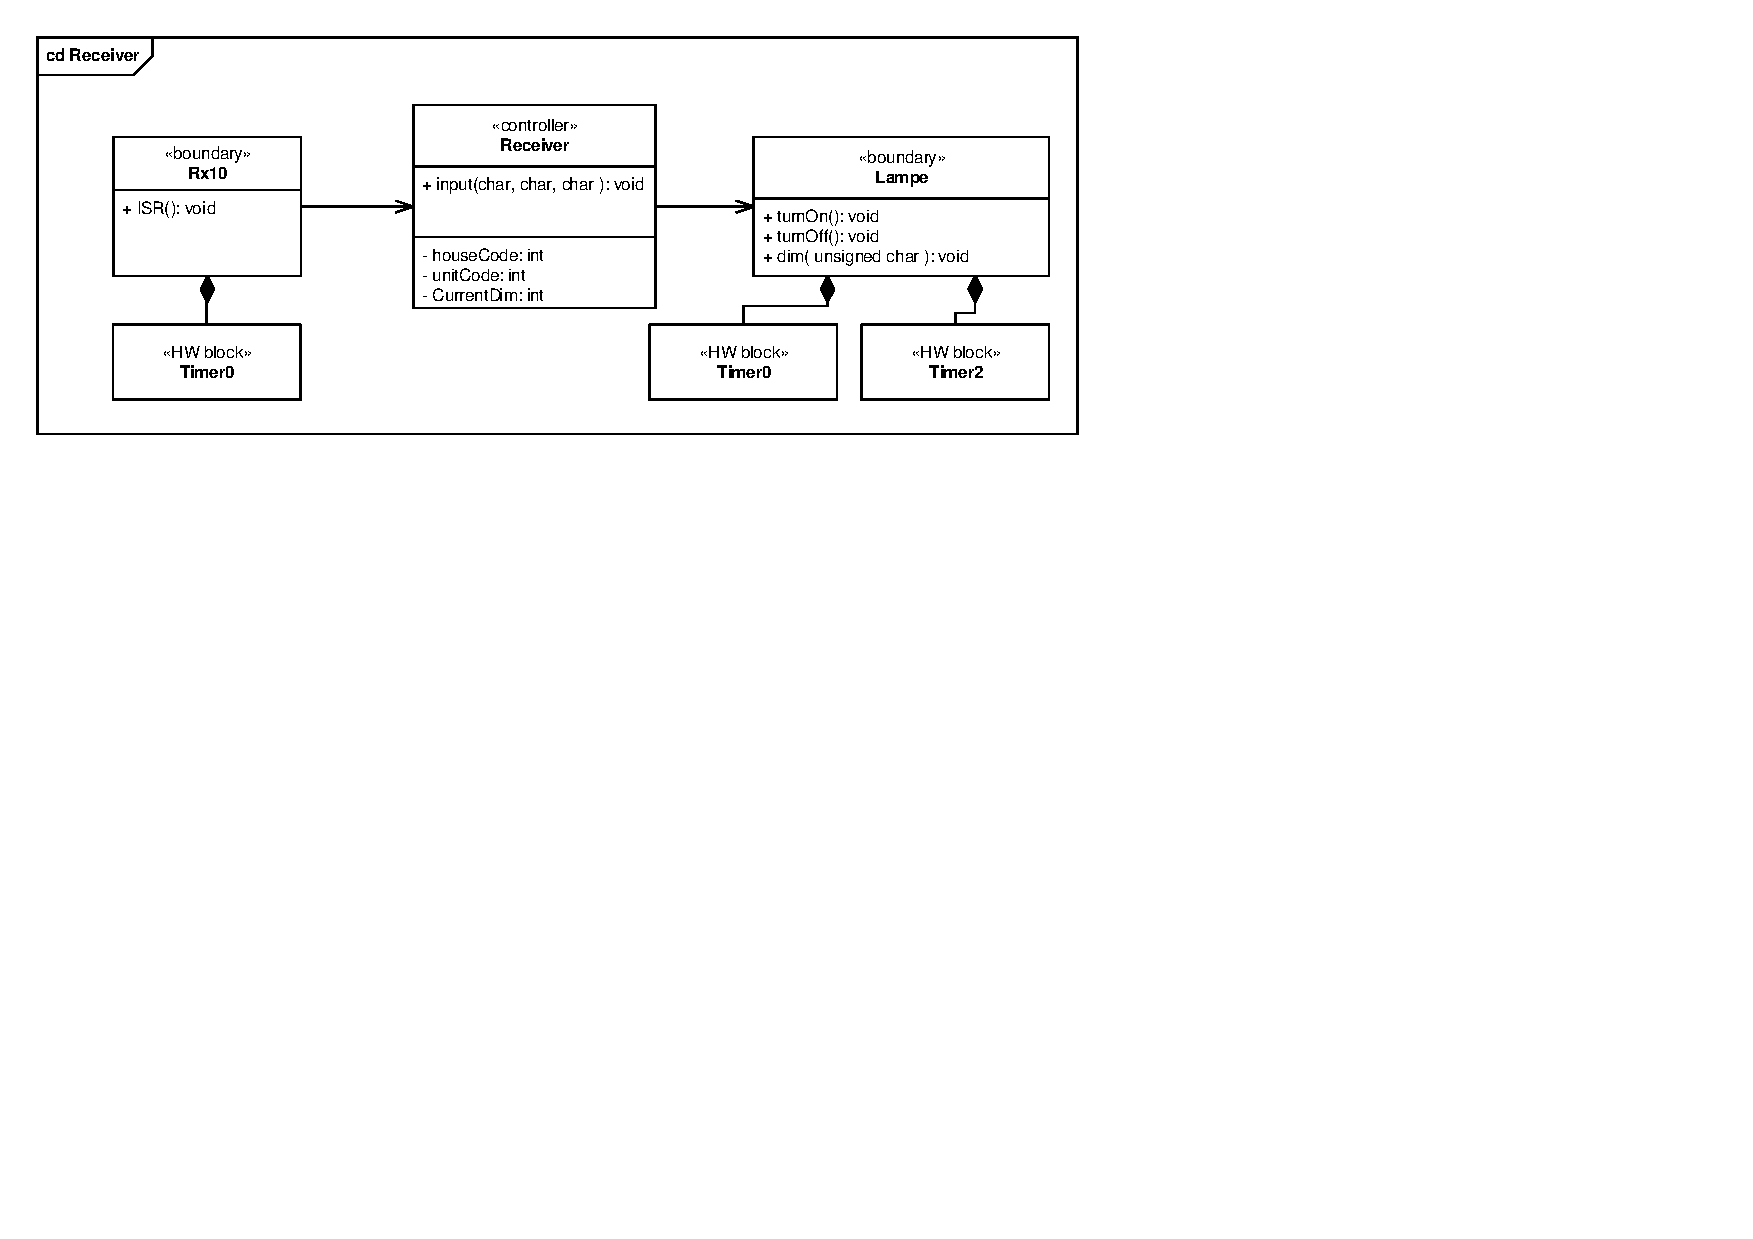
\includegraphics[scale=1,clip=true, trim=361.8 462 335 50]{Systemarkitektur/diagrammer/Receiver_KlasseDiagram} %L B R T - HUSKE DET
\end{figure}

\begin{table}[h]
\begin{tabularx}{\textwidth}{p{0.6 cm} l X} %\hline

%turnOn
\multicolumn{3}{l}{\textbf{turnOn}}\\
& Operation: & %Skriv tekst herunder
\texttt{void turnOn( void )}
\\ & Parametre: & %Skriv tekst herunder
Ingen.
\\ & Returværdi: & %Skriv tekst herunder
Ingen.
\\ & Beskrivelse: & %Skriv tekst herunder
Sætter PWM for lampen til 100\%.

\\ \end{tabularx}
\end{table}

%turnOff
\begin{table}[h]
\begin{tabularx}{\textwidth}{p{0.6 cm} l X} %\hline

\multicolumn{3}{l}{\textbf{turnOff}}\\
& Operation: & %Skriv tekst herunder
\texttt{void turnOff( void )}
\\ & Parametre: & %Skriv tekst herunder
Ingen
\\ & Returværdi: & %Skriv tekst herunder
Ingen
\\ & Beskrivelse: & %Skriv tekst herunder
Sætter PWM for lampen til 0\%.

\\ \end{tabularx}
\end{table}

\clearpage

%dim
\begin{table}[h]
\begin{tabularx}{\textwidth}{p{0.6 cm} l X} %\hline

\multicolumn{3}{l}{\textbf{dim}}\\
& Operation: & %Skriv tekst herunder
\texttt{void dim ( char )}
\\ & Parametre: & %Skriv tekst herunder
Modtager en char med en char med den ønskede dimnings værdi.
\\ & Returværdi: & %Skriv tekst herunder
Ingen
\\ & Beskrivelse: & %Skriv tekst herunder
Modtager en char som har en værdi mellem 0 og til og med 9, hvor 0 = 5\%, 1 = 15\% osv. Skal herefter ændre pulsbredden på det ben der er forbundet til lampen i forhold til den ovenfor angivne procent.
\\ \end{tabularx}
\end{table}

\subsection{Receiver (David)}

\begin{figure}[h]
\centering
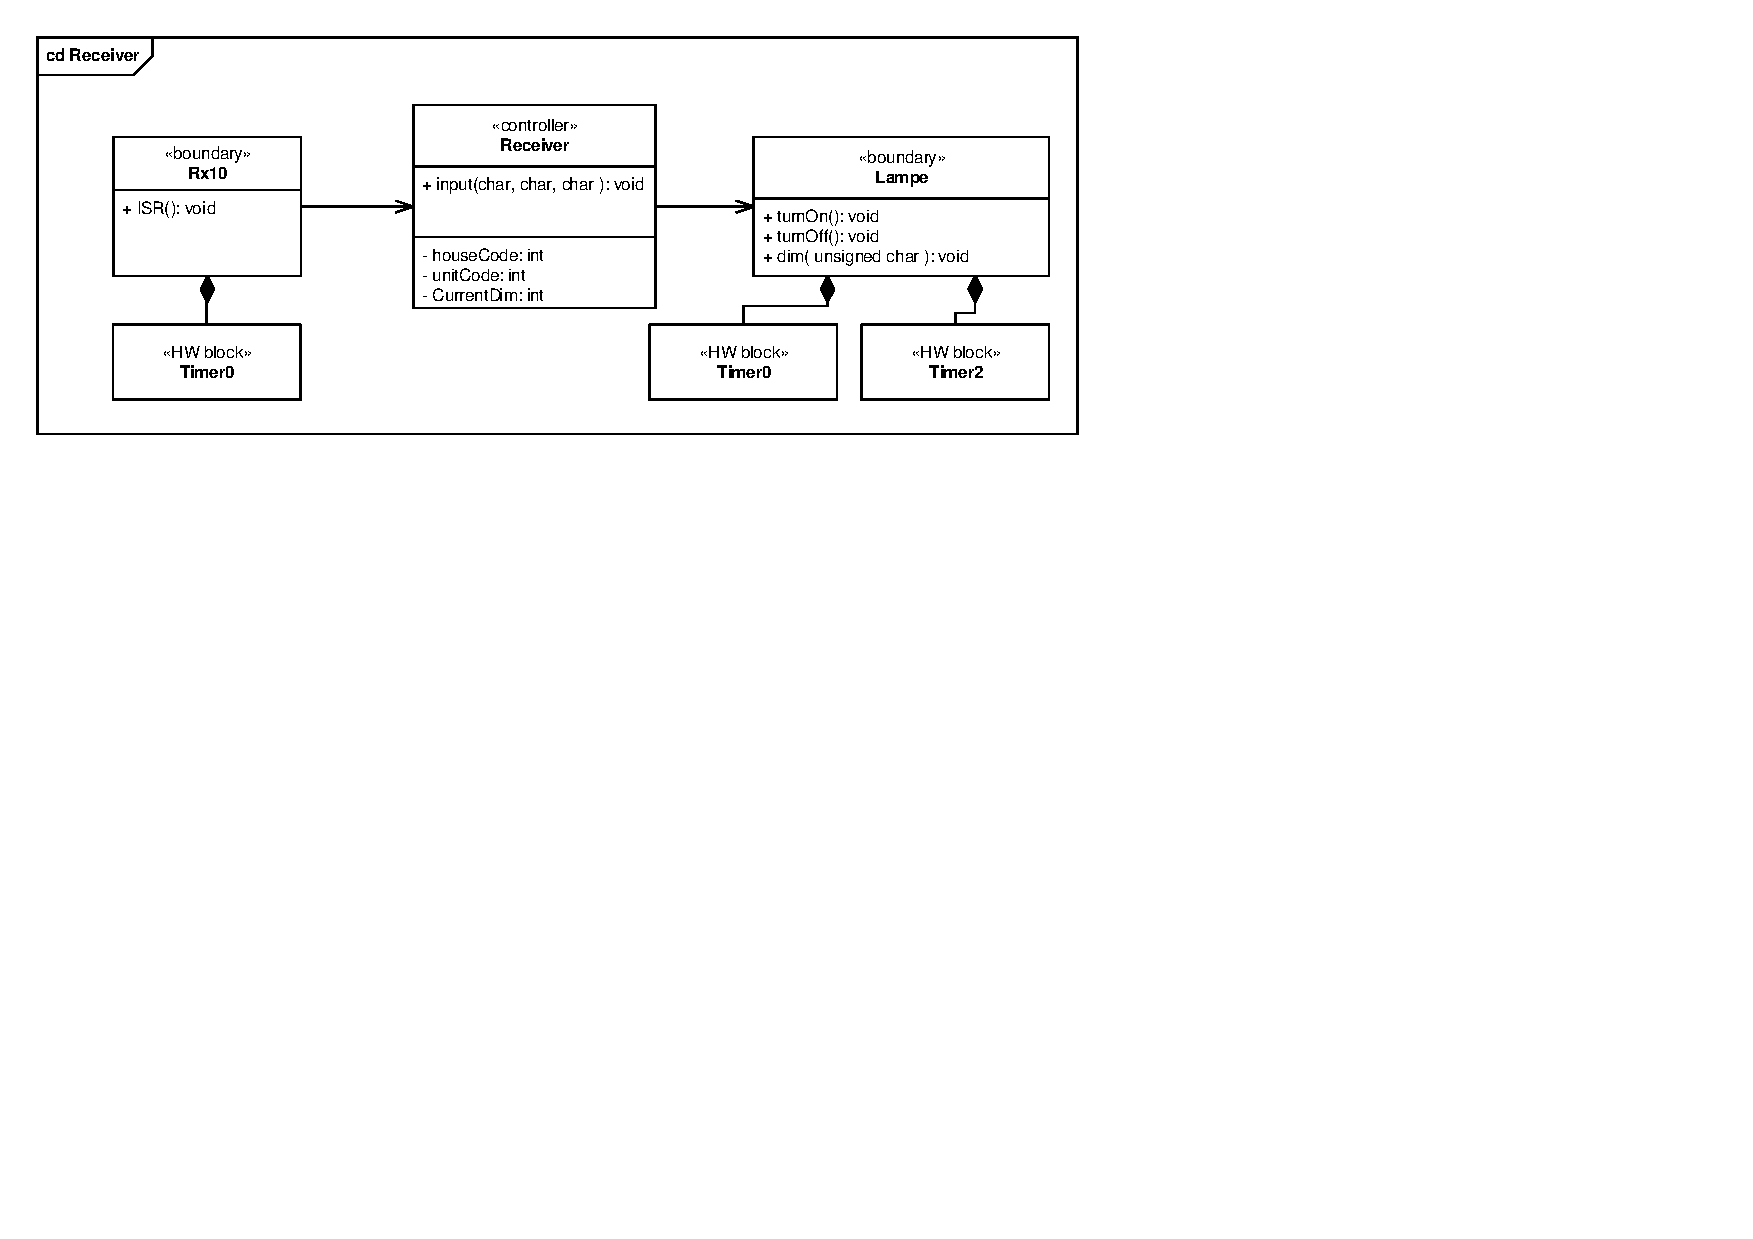
\includegraphics[scale=1,clip=true, trim=198 440 527 50]{Systemarkitektur/diagrammer/Receiver_KlasseDiagram} %L B R T - HUSKE DET
\end{figure}

\begin{table}[h]
\begin{tabularx}{\textwidth}{p{0.6 cm} l X} %\hline
\multicolumn{3}{l}{\textbf{Receiver}}\\
& Operation: & %Skriv tekst herunder
\texttt{void input( char )} 
\\ & Parametre: & %Skriv tekst herunder
Modtager en char fra X.10 som bruges til at finde om lampen skal. Tænde, slukke, dime op, eller dime ned.
\\ & Returværdi: & %Skriv tekst herunder
ingen retur værdi. 
\\ & Beskrivelse: & %Skriv tekst herunder
Controller for receiveren. Holder styr på lampen nuværerne dimning samt dens houseCode og unitCode.
\\ \end{tabularx}
\end{table}

\begin{table}[h]
\centering
\begin{tabularx}{13 cm}{|l |X|} \hline
Attribut & Beskrivelse \\ \hline

houseCode & Indeholder hus koden for denne Receiver \\ \hline
unitCode  & Indeholder unit koden for denne Receiver \\ \hline
CurrentDim & Den nuværerne dim værdi. \\ \hline

\end{tabularx}
\end{table}

\clearpage

\subsection{Rx10 (Kristian T.)}

\begin{figure}[h]
\centering
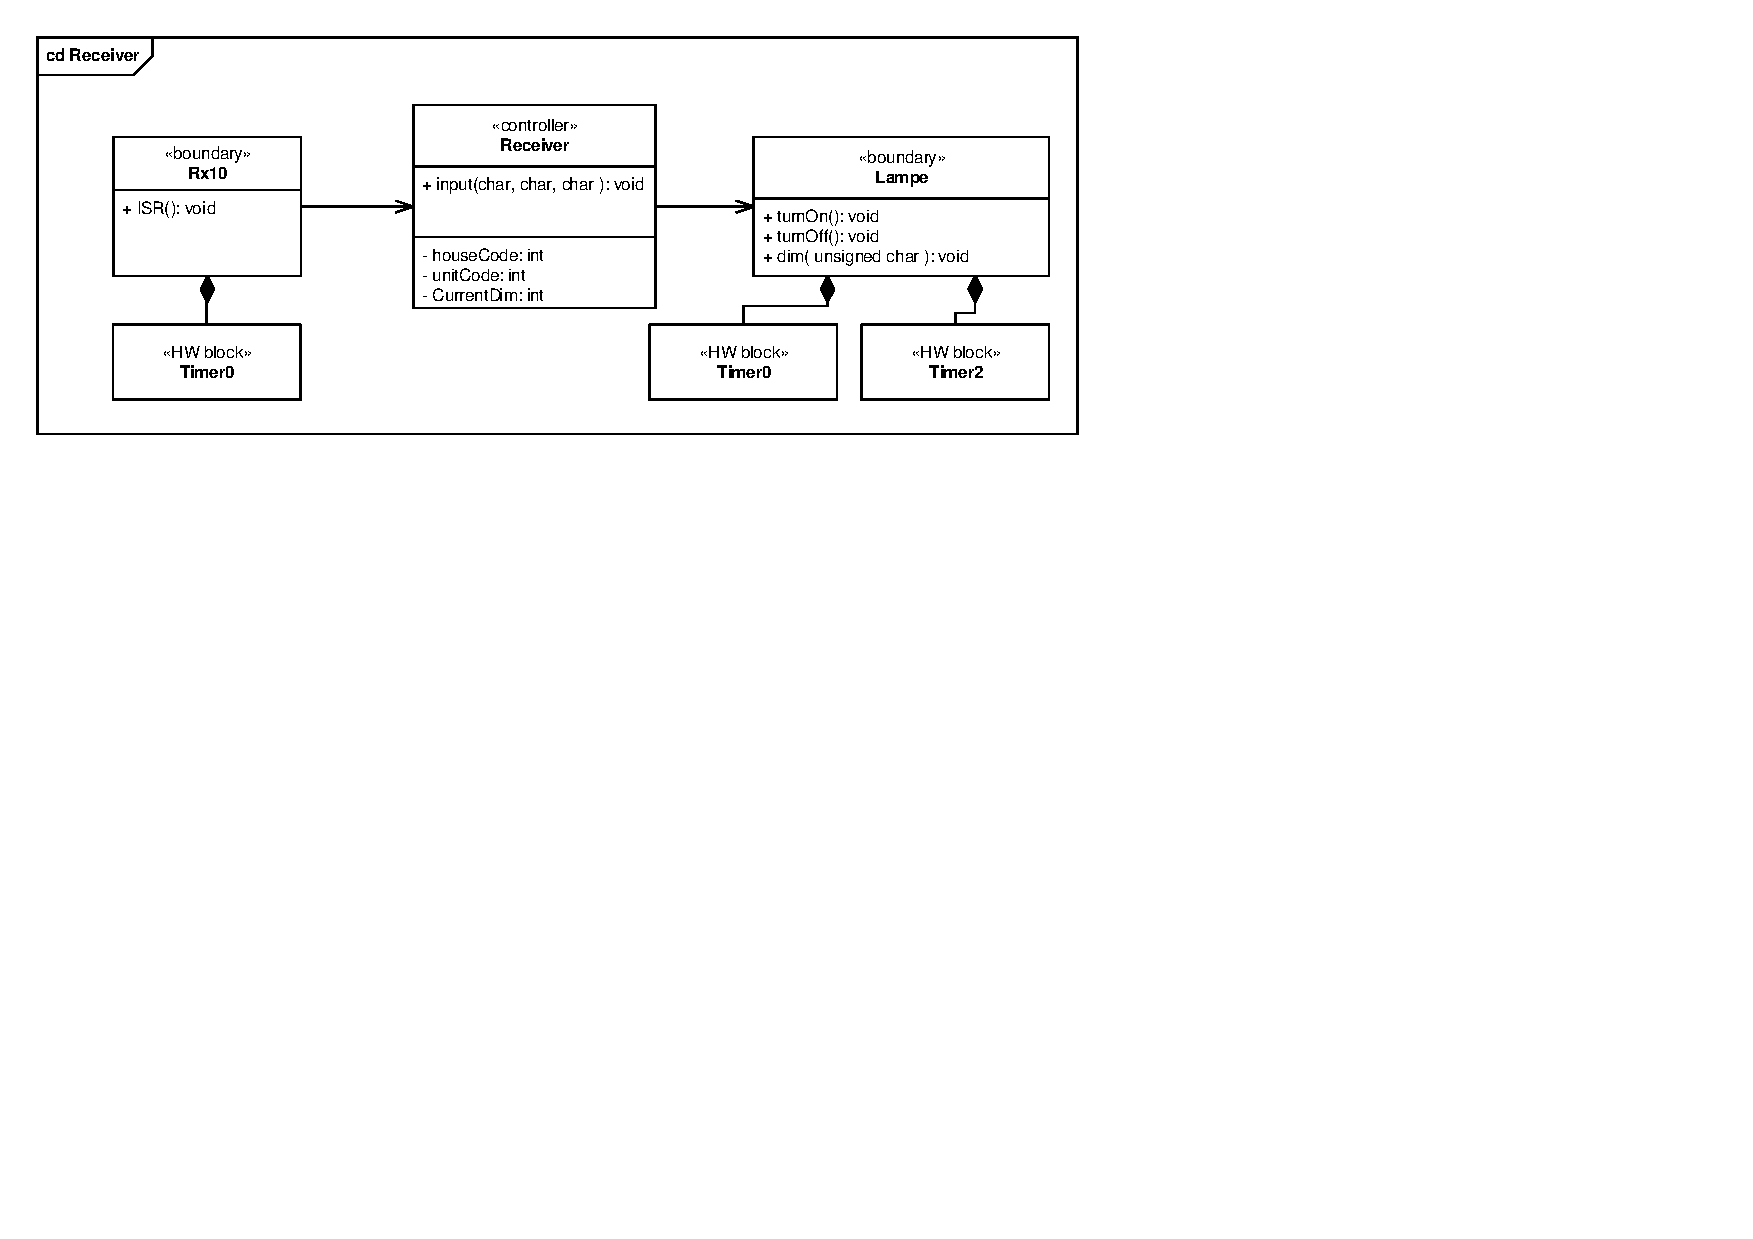
\includegraphics[scale=1,clip=true, trim=38 462 696 66]{Systemarkitektur/diagrammer/Receiver_KlasseDiagram} %L B R T - HUSKE DET
\end{figure}

%ISR
\begin{table}[h]
\begin{tabularx}{\textwidth}{p{0.6 cm} l X} %\hline
\multicolumn{3}{l}{\textbf{ISR}}\\
& Operation: & %Skriv tekst herunder
\texttt{ISR( INT0\_vect )}
\\ & Parametre: & %Skriv tekst herunder
Denne servicerutine er indbygget i Atmega32's IO bibliotek og modtager ingen parametre \cite{lib:AtMega32sum}.
\\ & Beskrivelse: & %Skriv tekst herunder
Denne funktion kaldes ved interrupts på \texttt{PD2 INT0} og skal være \texttt{Friend} af klassen. Ved interrupts skal denne skifte den nuværende værdi på PA0 ind i \texttt{temp}. Der udføres udføres herefter forskellige handlinger afhængigt tilstanden.
\\
\end{tabularx}
\end{table}

%checkData
\begin{table}[h]
\begin{tabularx}{\textwidth}{p{0.6 cm} l X} %\hline
\multicolumn{3}{l}{\textbf{checkData}}\\
& Operation: & %Skriv tekst herunder
\texttt{bool checkData( unsigned char )}
\\ & Parametre: & %Skriv tekst herunder
Modtager 8 nulgennemgange.
\\ & Returværdi: & %Skriv tekst herunder
Returnerer \texttt{TRUE}, hvis de 8 nulgennemgange overholder protokollen for 4 bits og \texttt{FALSE}, hvis den ikke gør.
\\ & Beskrivelse: & %Skriv tekst herunder
Denne metode kontrolleer om en given 4-bit størrelse overholder X.10 protokollen. Der modtages 8 nulgennemgange, som deles op i 4 par. Hvert par udgør 1 bit. For at returnere \texttt{TRUE} skal hvert par bestå af ét 1-tal og ét 0.
\\
\end{tabularx}
\end{table}

%translate
\begin{table}[h]
\begin{tabularx}{\textwidth}{p{0.6 cm} l X} %\hline
\multicolumn{3}{l}{\textbf{translate}}\\
& Operation: & %Skriv tekst herunder
\texttt{unsigned char translate( unsigned char )}
\\ & Parametre: & %Skriv tekst herunder
Modtager en \texttt{char}, som repræsenterer 8 nulgennemgange.
\\ & Returværdi: & %Skriv tekst herunder
Returnerer en \texttt{char} bestående af \texttt{0000} efterfulgt af de 4 bits, som inputtet oversættes til.
\\ & Beskrivelse: & %Skriv tekst herunder
Metoden tager parameteren og oversætter den til 4 bits. For at fylde \texttt{char}'en sættes bit 7-4 til \texttt{0} i returværdien. Bit 3-0 på returværdien sættes til bit 7, 5, 3 og 1 fra parameteren. 
Dvs hvis metoden kaldes med en char \texttt{10011010} vil returværdien være: \texttt{00001011}. 
\\
\end{tabularx}
\end{table}

\begin{table}[h!]
\centering
\begin{tabularx}{13 cm}{|l |X|} \hline
Attribut & Beskrivelse \\ \hline

\texttt{bool start} & Sættes til \texttt{TRUE}, hvis den er igang med at modtage en kommando, ellers sættes den til \texttt{FALSE}. \\ \hline
\texttt{unsigned char count} & Tæller hvor mange nulgennemgange der har været siden sidste hele bit/mønster. \\ \hline
\texttt{unsigned char temp} & Variabel som agerer skifteregister ved modtagelse af nulgennemgange. \\ \hline
\end{tabularx}
\end{table}

\clearpage